\documentclass[final,hyperref={pdfpagelabels=false},mathserif]{beamer}
\usepackage[]{color}
\usepackage{pdfcolmk}
\usepackage{eulervm}
\usepackage{tikz}
\usepackage{rotating}
\usepackage[scaled]{helvet}
\usepackage{epstopdf}
\usepackage{physics}
\usepackage{pgfplots}
\pgfplotsset{compat=1.8}
\usepackage[table]{colortbl} % table cell colours
\usepackage{hyperref}
\usepackage{graphicx} % Allows including images
\usepackage{booktabs} % Allows the use of \toprule, \midrule and \bottomrule in tables
\usepackage{physics}
\usepackage{tikz}
\usepackage{pgfpages}
\usepackage{caption}
\usepackage{float} % for [H] placement
\usepackage{enumitem}
\usepackage{tcolorbox}

%\usepackage[cmbright]{sfmath}
\mode<presentation>
  {
  \usetheme{ChR}
  \setbeamertemplate{bibliography item}[text]
}
  \usepackage{amsmath,amsthm, amssymb, latexsym}
  %\boldmath
  \usepackage[english]{babel}
  \usepackage[utf8x]{inputenc}
  \usepackage[orientation=portrait,size=a0,scale=1.3,debug]{beamerposter}

  % user defined
\newtheorem*{ans}{Ansatz}
\newcommand{\e}{\varepsilon}
\newcommand{\mathbox}[2]{
    \begin{beamercolorbox}[wd=\textwidth,rounded=true,shadow=true,left]{mathbox title}
        \textbf{#1}
    \end{beamercolorbox}

    \begin{beamercolorbox}[wd=\textwidth,rounded=true,shadow=true,left]{mathbox body}
        #2
    \end{beamercolorbox}
}
%  \renewcommand{\arraystretch}{0.7}
  \setlength{\parindent}{0 pt}
  \setlength{\parskip}{0 pt}

  \usepackage{booktabs}
  \renewcommand{\arraystretch}{1}
  \usepackage{array}
  % um Tabellenspalten mit Flattersatz zu setzen, muss \\ vor
  % (z.B.) \raggedright geschuetzt werden:
  \newcommand{\PreserveBackslash}[1]{\let\temp=\\#1\let\\=\temp}
  \newcolumntype{L}[1]{%
    >{\PreserveBackslash\raggedright\hspace{0pt}}p{#1}%
  }
  \usepackage[subfigure]{ccaption}
  \usepackage[FIGBOTCAP]{subfigure}
  \usepackage{multicol}
\usepackage{achemso}
\usepackage{caption}
\captionsetup{font=scriptsize,labelfont=scriptsize}
\setbeamertemplate{caption}[numbered]
\usetikzlibrary{calc,positioning,shapes.geometric,shapes.symbols,shapes.misc,calc,arrows,decorations.pathmorphing,intersections,decorations.pathreplacing,calligraphy}

\usetikzlibrary{decorations.pathreplacing}
\tikzset{
mybrace/.style={decorate,decoration={brace,aspect=#1}}
}
\newcommand*{\citen}[1]{%
  \begingroup
    \romannumeral-`\x % remove space at the beginning of \setcitestyle
    \setcitestyle{numbers}%
    \cite{#1}%
  \endgroup   
}

%%%%%%%%%%%%%%%%%%%%%%%%%%%%%%%%%%%%%%%%%%%%%%%%%%%%%%%%%%%%%%%%%%%%%%%%%%%%%%%%%5
\graphicspath{{figures/}}
\title{Boosted Imaginary Time Evolution of Matrix Product States}
\author{Benjamin C. B. Symons, Dilhan Manawadu, David Galvin, and Stefano Mensa}
\institute{The Hartree Centre, STFC, Sci-Tech Daresbury, Warrington WA4 4AD, United Kingdom}
  %%%%%%%%%%%%%%%%%%%%%%%%%%%%%%%%%%%%%%%%%%%%%%%%%%%%%%%%%%%%%%%%%%%%%%%%%%%%%%%%%5
  %% sensible column widths: 81cm (1 column);
  %%%%%%%%%%%%%%%%%%%%%%%%%%%%%%%%%%%%%%%%%%%%%%%%%%%%%%%%%%%%%%%%%%%%%%%%%%%%%%%%%5

\begin{document}
\vskip-1.4cm
%
% Übergeordnete Spalten
%
\begin{columns}[t]
%
% Spalte (1/3 der Seite) für Introduction, Experimental and Methods
% 
\begin{column}{40cm}
      
%
% Introduction 
%
\begin{block}{Imaginary Time Evolution}




\begin{itemize}[label=\textbullet, leftmargin=1em]
	\item 	Given a Hamiltonian $\hat{H} \ket{\phi_n} = E_n \ket{\phi_n}$, Imaginary Time Evolution (ITE) finds its ground state $\ket{\phi_0}$ by applying the non-unitary operator $\hat{T}={\rm{e}}^{-\hat{H}\tau}$ on some state $\ket{s} = \sum_{j} a_j\ket{\phi_j}$,

\begin{equation}
\ket{\psi(\tau)} = N(\tau) e^{-H \tau } \ket{s}
    = N(\tau) \sum_{j}e^{-E_j\tau} a_j\ket{\phi_j}, \notag
\end{equation}
where $N(\tau)$ is a normalisation constant.
	\item If $\braket{s}{\phi_0} \ne 0$, $\cfrac{\rm{e}^{-E_j\tau} a_{j \ne 0}}{\rm{e}^{-E_0\tau} a_0}$ decays exponentially with time, and therefore $\tau \rightarrow \infty, \ket{\psi(\tau)} \rightarrow \ket{\phi_0}$
%	\item By representing $\ket{s}$ as a Matrix Product State (MPS), ground state can be found via Time Evolved Block Decimation (TEBD).
%	\item Deep Trotterized circuits is a challenge for implementing ITE on (near-term) quantum computers.
\end{itemize}


\end{block}


\begin{block}{Boosted Imaginary Time Evolution (BITE) in 2D}

\begin{columns}[c]

 \column{.5\textwidth}
 
Performing ITE for $\Delta \tau$ on $\ket{s}$ gives
\begin{equation}
    \ket{t} = N(\Delta\tau) \left( e^{-E_0\Delta\tau}\ket{\phi_0} + e^{-E_1\Delta\tau}\ket{\phi_1}\right).
\notag
\end{equation}


\begin{tcolorbox}[colframe=blue!50!black, colback=blue!10!white, title=BITE Reflection Operator]
Defining the BITE reflection operator
\begin{equation}
    \hat{R}(\ket{v}) = 2\ket{v}\bra{v} - \hat{I}, 
\notag
\end{equation}
the $n^\mathrm{th}$ reflected state, $n \in \mathbb{N}$, is given by
\begin{equation}
    \ket{r_n} = \hat{R}(\ket{r_{n-1}}) \ket{r_{n-2}},
\notag
\end{equation}
where $\ket{r_0}=\ket{t}$.
\end{tcolorbox}

 \column{.45\textwidth}

\begin{figure}[H]
\centering
\begin{tikzpicture}[scale=10]
    \draw[->, ultra thick](0,0) -- (1,0) node (xaxis) [right] {$\ket{\phi_0}$};
    \draw[->, ultra thick](0,0) -- (0,1) node (yaxis) [above] {$\ket{\phi_1}$};
    \draw[->, thick](0,0) -- (0.70712,0.70712) node (sp) [right] {$\ket{s}$};
    \draw[->, thick](0,0) -- (0.806225,0.591609) node (t) [right] {$\ket{t}$};
    \draw[->, dotted, thick](0,0) -- (0.8866676622700842,0.462407070057131) node (r) [right] 
    {$\ket{r_1}$};
    \draw[->, dotted, thick](0,0) -- (0.9465712361839997,0.3224937765757464) node (b) [right] {$\ket{r_2}$};
    \draw[] (0,0) coordinate node (origin) [right] {};
\end{tikzpicture}
\caption{The state $\ket{r_1}$ is  produced by reflecting $\ket{s}$ about $\ket{t}$. The state $\ket{r_2}$ is  produced by reflecting $\ket{t}$ about $\ket{r_1}$.}
\label{const-2}
\end{figure}

\end{columns}

\end{block}

\begin{block}{Efficient boosting}
$\ket{r_n}$ is given by the recurrence relation
\begin{equation}
    \ket{r_n} = 2\braket{r_{n-1}}{r_{n-2}}\ket{r_{n-1}} - \ket{r_{n-2}} = 2\braket{t}{s}\ket{r_{n-1}} - \ket{r_{n-2}}. 
\notag
\end{equation}
\newline
As $\ket{r_n}$ is in the plane spanned by $\ket{s}$ and $\ket{t}$, one can write
\begin{equation}
    \ket{r_n} = \alpha_n\ket{t} + \beta_n\ket{s},
\notag
\end{equation}
with the recurrence relations
\begin{equation}
    \alpha_n = 2\braket{t}{s}\alpha_{n-1} - \alpha_{n-2}, \text{ and }
    \beta_n = -\alpha_{n-1}, 
\notag
\end{equation}
with the initial conditions $\alpha_{-1} = 0$ and  $\alpha_0 = 1$. It follows that the homogeneous recurrence relation for $\ket{r_n}$ has the close form expression

\begin{equation}
    \ket{r_n} = \frac{1}{\sin(\theta)}\left( 
    \sin((n+1)\theta) \ket{t} - \sin(n\theta)\ket{s}
    \right), 
\notag
\end{equation}
\vskip -5pt
where $\cos(\theta)=\braket{t}{s}$.

%\begin{equation}
%\begin{split}
%    E_n = \alpha_n^2 E_t + \alpha_{n-1}^2E_i - 2\alpha_n\alpha_{n-1}E_{it}.
%\end{split}
%\notag
%\end{equation}

\end{block}




\begin{block}{Stop criterion}
Energy of the $n^\mathrm{th}$ reflected state $\ket{r_n}$ is
\begin{equation}
\begin{split}
    E_n = \alpha_n^2 E_t + \alpha_{n-1}^2E_i - 2\alpha_n\alpha_{n-1}E_{it},
\end{split}
\notag
\end{equation}
where $E_t = \bra{t}\hat{H}\ket{t}$, $E_s = \bra{s}\hat{H}\ket{s}$ and $E_{st} = \bra{s}\hat{H}\ket{t}$.
\vskip 10pt

$E_n$ is calculated until $E_{n+1} > E_n$, and $\ket{r_n}$ is found using the closed form expression.

\end{block}

\begin{block}{BITE algorithm}

\begin{itemize}[label=\textbullet, leftmargin=*]
    \item Imaginary time evolve an initial state $\ket{s}$ by a single step $\Delta\tau$ to produce a state $\ket{t}$.
    \item Calculate the overlap $\braket{t}{s}$ and the terms $E_t$, $E_s$ and $E_{st}$ and the series of energies $E_n < E_{n+1}$. Compute the corresponding state $\ket{r_n}$.
    \item Imaginary time evolve $\ket{r_n}$ by a single step to produce a new initial state $\ket{s'}$, and by two steps to produce a new evolved state $\ket{t'}$.
    \item Repeat steps 1-3 using the new states $\ket{s'}$ and $\ket{t'}$ as the initial states until the energy converges.
\end{itemize}

\end{block}

   \begin{block}
{BITE in 3D}

\begin{columns}
    \begin{column}{0.5\textwidth}
        \centering
        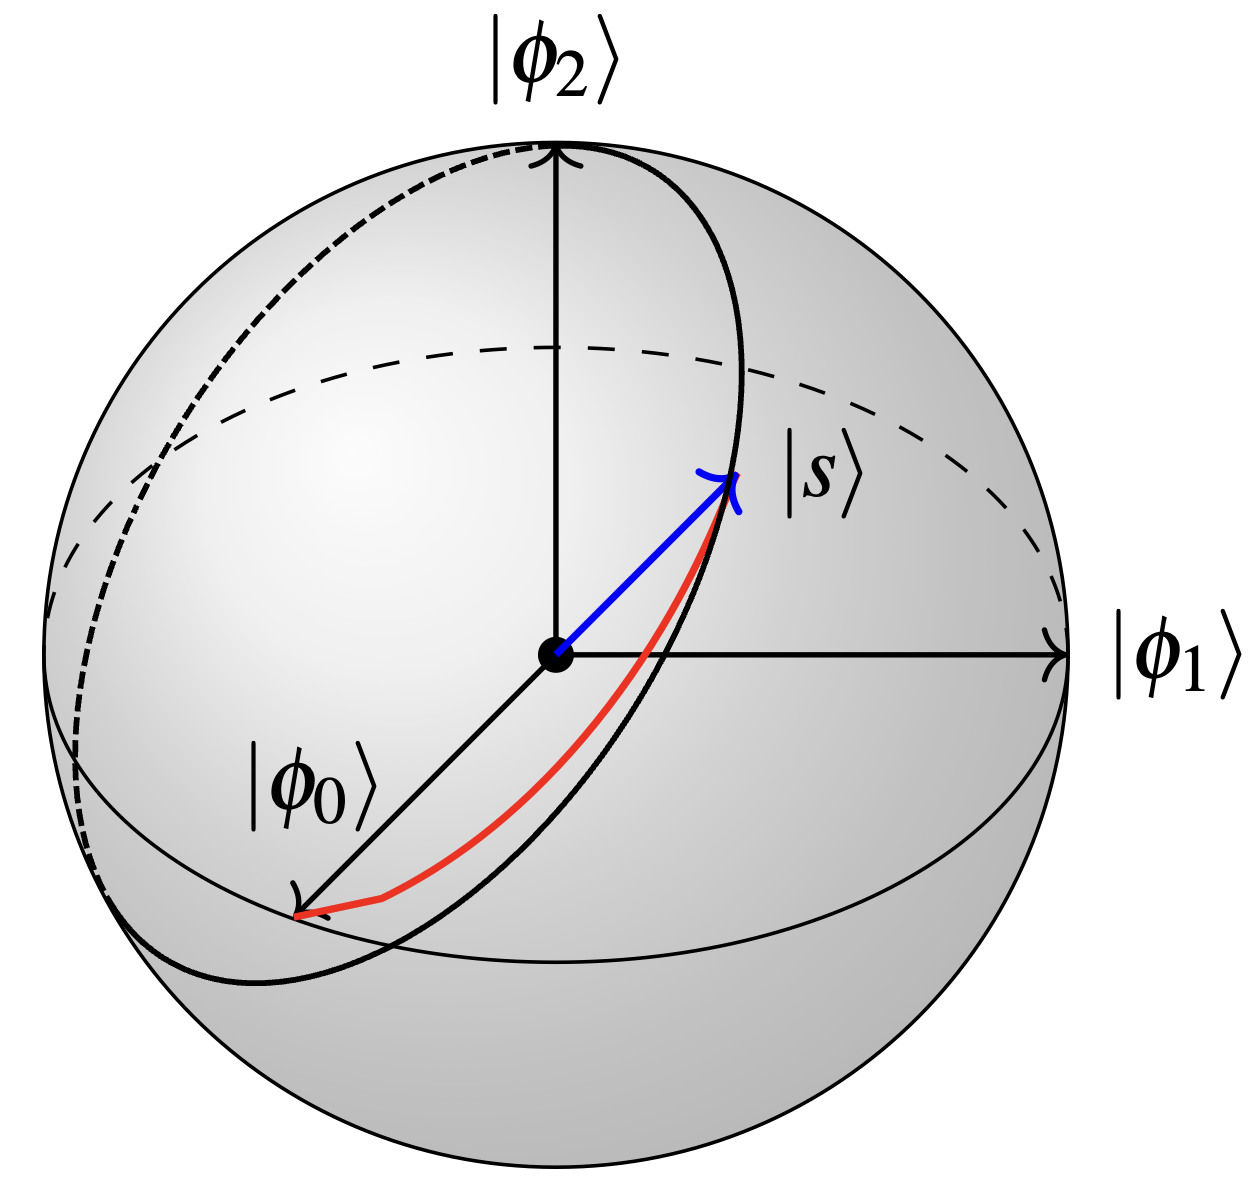
\includegraphics[width=0.75\textwidth]{sphere-bite.png}
    \end{column}
    \begin{column}{0.5\textwidth}
        \captionof{figure}{A visualisation of BITE in a norm conserving 3D Hilbert space. The blue vector represents the initial state $\ket{s}$ and the red curve is a trajectory resulting from imaginary time evolution. BITE can access any state on the the black great circle spanned by $\ket{s}$ and $\ket{t}$ (not shown).}
        \label{fig:sphere}
    \end{column}
\end{columns}

\end{block}
	


\end{column}

%\begin{column}{27cm}
%
%
%      
%%
%% Introduction 
%%
%
%
%\end{column}


\begin{column}{40cm}
     

%
% Introduction 
%
\begin{block}
{Results}

As a test case, we use the transverse field Ising model on a 1D spin chain given by
\begin{equation}
    \hat{H} = -J\sum_{i,j} X_i X_j -g \sum_{i}Z_i,
    \notag
\end{equation}
\vskip -5pt
with $n=100$ sites, open boundary conditions, $J=0.5$ and $g=1.5$, $\Delta \tau = 0.001$.
\vskip -5pt

\begin{figure}[H]
    \centering
    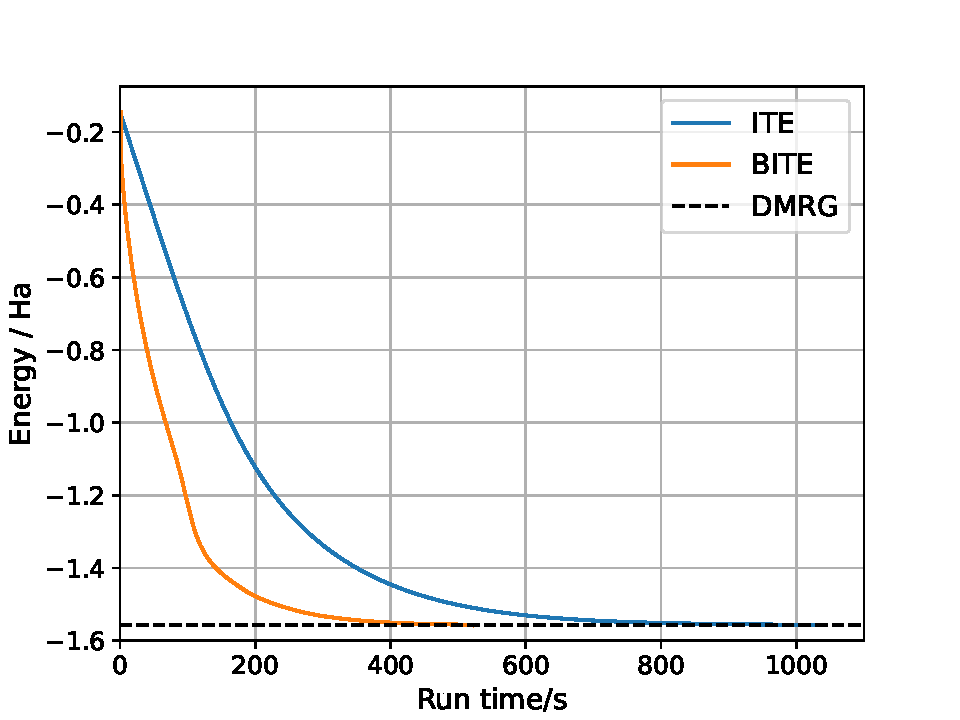
\includegraphics[width=0.79\textwidth]{Energy_tr_L100_dt0_001_g1_5_J0_5.pdf}
    \caption{The energy per site of the MPS vs run time for ITE and the BITE algorithms. Dashed black line is the DMRG energy.}
    \label{fig:energy}
\end{figure}

\begin{figure}[H]
    \centering
    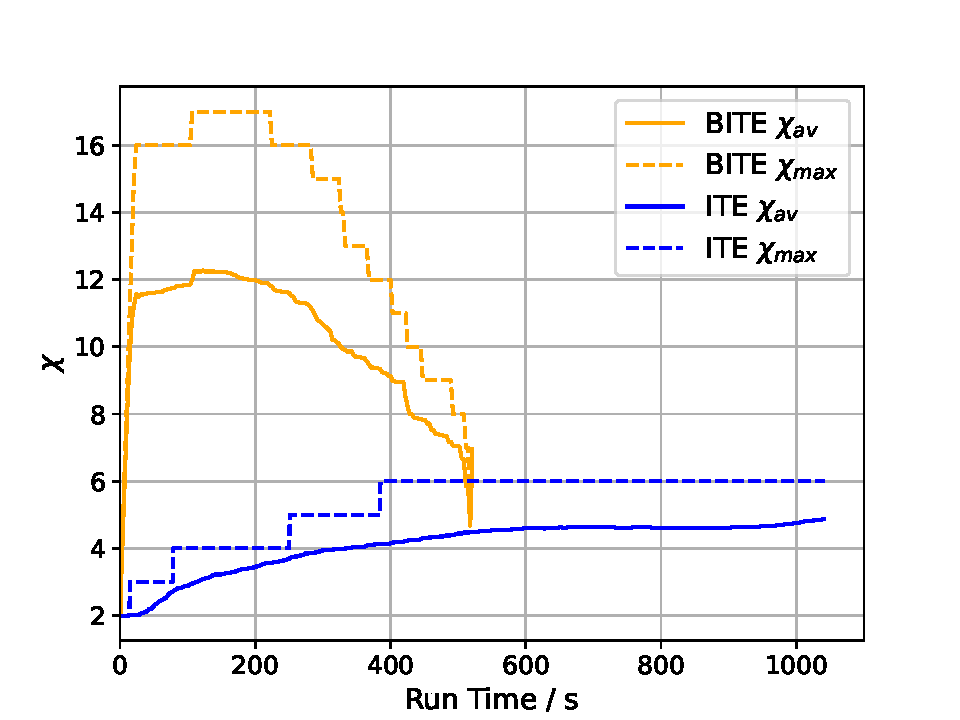
\includegraphics[width=0.79\textwidth]{Chi_tr_L100_dt0_001_g1_5_J0_5.pdf}
    \caption{Average and maximum bond dimension at each point in the BITE and ITE calculations. $\chi_{av}$ is averaged over all matrices in the MPS.}
    \label{fig:chi}
\end{figure}

\end{block}

\begin{block}
{Results}

\begin{table}[h]
\caption{Run time, maximum and average (over the entire calculation) bond dimension and fidelity of the final state with the ground state for various time step sizes.}\label{tab:table-1}
\centering
    \begin{tabular}{crrrrrr}
   \toprule
    Method & $\Delta\tau$ & $t_r$ & $\chi_{max}$ & $\chi_{av}$ & $|\braket{\phi_0}{\psi}|^2$ \\
   \midrule
    ITE & 0.001 & 1042 & 6  & 4.1 & 0.953 \\

    BITE & 0.001 & 521 & 17 & 10.2 & 0.998\\

    ITE & 0.005 & 204 & 7 & 4.5 & 0.956 \\

    BITE & 0.005 & 156 & 16 & 6.3 & 0.959 \\

    ITE & 0.01 & 105 & 7  & 4.8 & 0.960 \\

    BITE & 0.01 & 79 & 16 & 5.8 & 0.957 \\
\bottomrule
    \end{tabular}
\end{table}
\end{block}

\begin{block}
{Conclusions}
\begin{itemize}[label=\textbullet, leftmargin=*]
\item Here we present a novel quantum-inspired classical algorithm that has the potential to speed-up the convergence of imaginary time evolution of matrix product states to a ground state.
\item We have presented a proof-of-concept demonstration of the method applied to the 1D transverse field Ising model with open boundary conditions.
\item In this work we have focused on the 1D case where DMRG is typically a better method than ITE. However, it may be possible to extend the BITE method to 2D where the use of imaginary time evolution is more prevalent.
\end{itemize}
\end{block}

\begin{block}
{Acknowledgements}

This work was supported by the Hartree National Centre for Digital Innovation, a UK Government-funded collaboration between STFC and IBM.
\end{block}
\end{column}

\end{columns}

% Ende Poster Seite und Dokument!
%
\end{document}